This chapter presents the current state of the art in the domain and talks about other similar work that has been done in this area. It also establishes the novelty of our work by highlighting the differences between the existing work and our work.

\section{Purpose}
The purpose of this literature review is to study and analyze various researches related to the different components of the project to develop an understanding of the subject fields as well as what is required from the project as a whole. It is also an opportunity for us to constructively criticize other works that have been done in similar fields and/or technologies. AEGIS comprises of various concepts of Electrical Engineering and Computer Science, each idea diverse from the other. This literature review is thematically written to ease the division of literature subject-wise and allow for the identification of contradictions, similarities and emergence of ideas. 

\section{Existing Solutions}
\label{section:existingSolutions}
\begin{enumerate}
    \item An Indian start-up, HoloSuit has developed a product that can capture the entire body motion, including fingers, head and feet, and can transfer it to a robot or virtual character which can then be used in the virtual world. This HoloSuit is being used for several consumer and enterprise applications, including karate training, cricket training, yoga and many more. A human trainer may record the karate moves in the virtual world, and users can later learn from those recorded moves in the virtual world while the software constantly gives real time review on their performed moves, the haptic exciters closest to the discrepancy will vibrate to notify the user of any wrong move \cite{HoloSuit1}. This product is head to toe wearable and gives haptic feedback and one on one fight session. However it is not locally available and very expensive (4 lacs PKR).
    
    \item A Singapore based game studio, Gattai Games, has developed a VR Kungfu Simulator, where players can fight with enemies using their Kungfu skills while wearing a haptic suit that lets them feel the punches and other attacks from their enemies \cite{gattaiGames}. This is also provides haptic feedback but again it is not available in Pakistan and very expensive since it connects with Oculus rift. Hence, it is hardware dependent and costly. Furthermore it is just a game and does not provide any user review or feedback. 
    
    \item VR Self-defence is a free quick solution to learning self defence moves. It provides a virtual character (a dummy) for the user to practice a set of four moves on, only passing them if they hit all of the spheres correctly and quickly \cite{VRselfdef}. This solution also provides haptic feedback however, it lacks on providing one-on-one realistic sessions with a trainer, the user can not practice his learned skills with anyone. The interface and experience is very dull, the software only requires the user to practice on a dummy in a virtual world. It provides no feedback to the user on performed moves. No adaptivity, no levels.
    
    \item A postgraduate research based in California focuses on the use of VR technology along with passive haptics for the development of a military training system. The thesis is designed to look for and design a system for aerial attack and defence training, known as MANPADS (Man Portable Air defence Systems). This development will help provide a cost effective training course for military purposes \cite{manpads}. It provides haptic feedback to feel the impact. The product itself is versatile and covers various self defence and offence strategies. It covers the entire body from head to toe. It provides one-on-one realistic sessions with a trainer, the user can practice his learned skills with the trainer. However, it is not accessible to civilians, it is not available in Pakistan and it focuses on army training rather than self defence for civilians. It provides no feedback to the user indicating how he performed. 
    
    \item Other existing solutions include human trainers/institutes and YouTube videos that can be used to learn the art of fighting. Human trainers do not need haptic suites. A real experience is irreplaceable. A professional trainer gives the best feedback after practice sessions at the end of each training. Most of the human trainers teach in an adaptive style. However, high monthly fees and non-accessibility of trainers to many people due to various reasons are restrictions. Lack of women trainers is a reason why many women (who need self defence) are reluctant to attend these institutes. 
    
    Online courses do not offer any realistic experience at all, and most of these online courses do charge. There is absolutely no feedback provided and it is the least interactive of all the existing solutions with no practice sessions.
\end{enumerate}

\section{Haptics}
\label{section:hapticLit}
Haptic is a relatively recent technological advancement. It simulates senses of movement and touch to in turn, reproduce the sensations to be felt by a user indirectly as if interacting with physical objects; it is the sensation and manipulation through touch. Haptics uses the sense of touch to be able to display emotions, make technology interactive, experience virtual reality, smart surveillance, gaming, and much more \cite{affHaptics}. 


According to a research conducted by Institute of Electrical and Electronics Engineers (IEEE), effective haptics comprises of three main domains: effective computing, haptic interfaces and user experience. Effective computing detects, displays and explicitly communicates emotions \cite{affHaptics}. Effective computing combines ideas from fields of psychology, cognitive science, and computer science to ensure the smooth flow of the system without ethical concerns. Haptic interfaces provides communication of touch to and from a human subject.


Among the many applications of haptics, NeuroCuddl is one that incorporates both virtual reality and haptics into a biofeedback system for mental wellness \cite{neuroCuddl}. NeuroCuddl is a user interactive Virtual Reality (VR) environment for mental health and recreational experiences, unique for each user’s personal data and state. The program simulates muscles and provides relaxation by playing synthesized music and displaying dynamic visuals regulated by the user’s breathing pattern and mental state to serve as therapy and mental health treatment \cite{neuroCuddl}. Various aspects of NeuroCuddl are similar to those of our project. It includes a list of components used; this list is crucial for developing our list of essential components needed for the project. Not only that, it helped us understand how to shape our project hardware to match our requirements from both producer and user perspectives respectively.

\subsection{EMS and Other Force Feedback Techniques}

Since it is a relatively new field of exploration, haptics is widely known for its miniaturization gap, or the manufacturing of small mechanical parts and products. Electric Muscle Stimulation (EMS) not only fills the miniaturization gap, but also is able to deliver a wide range of tactile and force feedback. EMS is a wearable haptic technology that can be miniaturized and deliver a wide range of haptic output.


EMS, though extremely resourceful in haptics, has several safety precautions that need to be taken into account. EMS uses slight current on the user’s body to simulate "skin receptors and muscle fibers", hence there comes forth several hardware and software precautions users need to take to ensure safety \cite{toolkit}. The idea of setting up a calibration system for the user before proceeding to using EMS for the rest of the program derived from the varying levels of current from person to person. The calibration system guarantees safety of the user and hardware; asking the user for their preferred levels removes the chance of any disruption or damage. Keeping precautions in our mind, EMS restricts its users to those who it will not harm in any way. People who have a heart disease, pregnant women, people with epilepsy, skin disease or cancer, and those who have recently gone through surgery should not use EMS devices.


A method of providing force feedback eliminates the incorporation of motors and mechanics. This method is substantially smaller and requires a lot less energy than other previously used methods. It actuates the users’ forearm muscles using four electrodes, which causes the muscles to contract involuntarily. Resistance of motion of the arm allows the user to perceive force feedback \cite{muscleForceFeedback}. Force feedback is preferred over vibrotactile in applications like enabling eyes-free targeting, increasing task realism, and enhancing immersion in video games because it provides physical forces that counter the users’ movements. The proposed idea of bringing force feedback to mobile devices will function using the user’s muscle power and EMS. Its approach achieves miniaturization by eliminating mechanical actuators like motors, and substantially reducing battery size. Setting up the device for the technology is manual placement of electrodes, which require knowledge on the proper placement and timing of the project. 


Other method for force feedback is motor-based, where force feedback devices administer force to body joints mechanically. Another method is a non-rigid actuation that includes transmission of force through sound pressure or pneumatic systems (example air jets) \cite{muscleForceFeedback}.

A recent paper on “Novel digital glove design for virtual reality applications” tells us about technological needs for designing haptic wearables that contain both impact and force feedback. Our project needs both of these \cite{NovelGlo}. A recent project by the name Dexmo is developing an exoskeleton for motion capture and forced feedback \cite{Dexmo}. Although Dexmo is lightweight and inexpensive, it provides binary feedback, and our aim is to make sensation a little realistic by adding levels to it rather than restricting it to binary haptic feedback. Yet another paper presented a new approach to rendering the haptics of heavy and stationary objects, in particular by means of electrical muscle stimulation \cite{EMSLopes}. For haptics it can be servo vs high torque motors, EMS vs vibrational motors. There are a number of researches that show superiority of EMS over the use of high torque motors and vibrotactile actuators. 

\subsection{Haptic Calibration}

EMS is a well-suited technology for providing haptic feedback for free-hand interactions, or hand movements and tactile stimuli, to receive feedback with specific information or characteristics. A few of such characteristics involved in haptic feedback is strength, pattern, velocity, etc. 
The numerous use cases of interactions requiring or benefiting from haptic technology include home entertainment, gaming, and can go as beyond as surgical information displays like X-rays. Haptic feedback is beneficial to indicate that an action has been performed; the technology stimulates different nerves and receptors in the human skin, which gives the user feedback through vibration. It is different from mobile phone feedback, which gives a sense of vibration when in contact with the screen.  An accessible form of receiving haptic feedback is through wearable devices that can emit EMS feedback, such as wristbands. Wristbands are not a novel idea, since many fitness and massage systems have launched wristband devices for their respective purposes that are controlled in hand, too \cite{emsDesign}.  


Haptic sensing capabilities are based on the nerves in the skin, tissue and muscle that are stimulated by touch, pressure and heat. Exact measurements for electrical impulses longer than 10ms are as follows: current of 10-20 mA to stimulate the sensory nerve fibers, additional 20-40 mA stimulates the motoric nerve fibers, and of more than 40 mA stimulates the pain nerve fibers. These measurements for density of nerves vary depending on the body position. The amount of current that gets through the skin is defined by the size of the conductive area and the conductivity of the electrodes. The more current applied, the more skin receptors are stimulated. Applied current can be induced using actuators placed on the skin or other parts of the body. 


Characteristics that influence the haptic perception in terms of current applied includes the strength of applied current, applied duration, impulse form, impulse frequency, and impulse duration. The form of impulse mostly follows characteristics of a sine wave, a square wave, or a saw tooth wave. EMS typically uses frequencies between 1 Hz and 1 kHz. With short impulses of 100 us the skin resistance decreases and with long pulse duration the skin resistance increases. For contacting a muscle, impulse duration of up to 400 us are typically used \cite{emsDesign, toolkit}. There are a number of variations of positioning the EMS on the body that result in different muscles being stimulated, each depending on the action for which feedback should be applied. 

\section{Pose Estimation and Evaluation}
\label{section:openposeLit}
\subsection{Pose Estimation using Openpose}
Pose estimation is a technique that detects human figures using input images and/or videos to determine the coordinate location of certain body parts. For our project, pose estimation is required in order to detect the movement of the user. The pose estimation is used to determine the specific pose of the user at a particular frame for future evaluation and analysis. Several applications are able to use detected key points for further applications like mesh reconstruction, but OpenPose is the only existing method that can provide whole-body pose estimation with relative accuracy \cite{wholebodyPoseEst}. OpenPose's runtime is proportional to the number of people in the image, which means that whole-body estimation becomes extremely costly  for multiple people at the same time \cite{wholebodyPoseEst}. A technique to resolve this problem is to resort to multi-task learning (MTL). However, since our project only works to detect a single person, it does not require this particular feature to be available. 


There are two known approaches to detect body landmarks and face alignments: template fitting and regression-based. Template fitting cascades regression functions and builds face templates to fit previously-set input images. Regression method, contrarily, applies convolutional heat-map regression on Convolutional Neural Networks (CNNs) \cite{wholebodyPoseEst}. Openpose uses CNN to ensure accuracy in each pose detection. With CNNs, there are massive annotated datasets (COCO and MPII) released whose results for single-person estimation is even more accurate. Several existing body keypoint detectors are not integrated with the libraries used for the specific functions. OpenPose, on the other hand, overcomes these problems as it can run on different operating platforms like Ubuntu, Windows, Mac, OSX, and Nvidia \cite{wholebodyPoseEst}. It is also accepting of different hardware types like CUDA GPUs, OpenCL GPUs and CPU-only devices. In addition to that, users have the freedom of choosing between images, video, webcam and IP camera streaming as input data provider. 

\subsection{Datasets for Pose Estimation}
There are two popular human pose datasets that contain an array of points representing different points on the body: MPII and COCO. The MPII dataset contains 15 of such points, which COCO contains 18. For our project, we are using the COCO dataset because it is far more accurate than the former \cite{wholebodyPoseEst}. There exist a dataset COCO+foot (Body 25 dataset) that contains the mutual 18 body points and additional feet points. This particular dataset is not needed for our application, hence to avoid the slowing of devices, we chose the regular COCO dataset. Below is an example of COCO keypoint format used for human pose.

\begin{figure}
\centering 
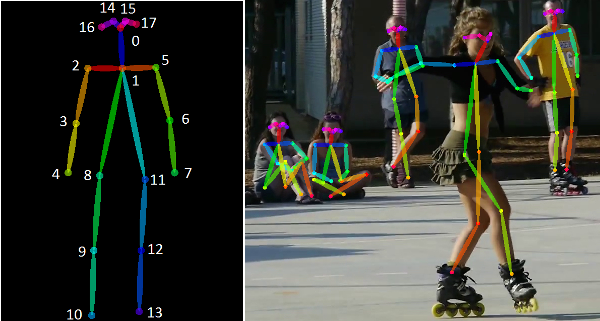
\includegraphics[scale=0.5]{images/COCO.png}
\caption{Pose Estimation using COCO dataset}
\end{figure}

\subsection{Pose Evaluation and Scoring}
Scoring is an essential component of the project. It is a measure of how the user is performing in comparison to the dataset of benchmark videos that are accurate moves. The scoring algorithm uses the dataset videos and its respective generated keypoints and compare the keypoints of the moves made by the user with the benchmark. Movements made by the users can be characterized by different qualities, like spatial and temporal perturbations of the movement \cite{movementQuality}. Computational analysis of user movement can be measured using Bio-mechanical efficiency, shape, and Intrapersonal synchronization, including aspects like postural control, coordination and balance \cite{movementQuality}. The same set of characteristics are used to judge dance (gymnastics, ballet), crafting (pottery), yoga, and various other sports. 


Biomedical efficiency helps in making movements avoid wastage of energy by trying to maintain maximum effectiveness. Shape relates to the posture of the movement performed; whether a particular posture was maintained throughout the frame or not. Lastly, Intrapersonal Synchronization focuses on body limb coordination with respect to the time between the movement of different body parts; checking whether two arm or legs move synchronously respectively is intrapersonal synchronization \cite{movementQuality}. 


For the scoring and evaluation of the performed moves, a similar research has been done on evaluating the gymnastic movements by assigning judgement scores through an algorithm which extracts detailed velocity field information from body movements (collected through a live performance video) and transforms them into specialized spatio-temporal image templates. The collection of such images over time, when projected into a velocity covariance eigenspace, trace out unique but similar trajectories for a particular gymnastic movement type. By comparing separate executions of the same atomic gymnastic routine, their method assigns a quality judgement score that is related to the distance between the respective spatiotemporal trajectories. For several standard gymnastic movements, the method accurately assigns scores that are comparable to those assigned by expert judges. \cite{gymnastic}
 

Another research focused on evaluating the effectiveness of a performed move through the relative position of joints. The skeletal data of a human is represented in an angular representation where each angle is defined by three joints and each joint is a 3D coordinate. The calculated angle is used to calculate the cosine similarity between the two aligned sequences. \cite{Karate}


Idris in \cite{Idris} also discusses an EF (extrinsic feedback) based approach to automate an evaluation system to evaluate the effectiveness of performed Martial Arts techniques.
 

A recent research conducted in 2019 presents a computational framework for automating the process of measuring movement quality in full body physical activities. Starting from motion capture data, the framework computes low-level (e.g. limb velocity) and high-level (e.g. synchronization between different limbs) movement features. Then, this vector of features is integrated to compute a value aiming at providing a quantitative assessment of movement quality, approximating the evaluation an external expert observer would give of the same sequence of movements \cite{movementQuality}. Pose Trainer \cite{poseCorrect} is an application that acts as a virtual workout trainer. It captures user's motion and compares it with stored dataset. It returns what went wrong in the pose. 




